\lhead{\emph{Implementation}}
\chapter{Implementation}
This chapter describes the different components of the Spatial Music Menu system. The main components includes a headset interface and an iOS application controlling the headset.


\section{Headset}
The headset interface used in this project is the Intelligent Headset (IHS)\footnote{\url{https://intelligentheadset.com/}}. The headset uses HRTF technology and can deliver spatial audio. 4 sensors are built into the headset; GPS, compass, gyroscope and accelerometer - making it possible to track head rotation and location of the user wearing it. The headset also includes 2 buttons - one in the outer center on each speaker. Connection to the headset is accessible via Bluetooth or wire. The headset is shown in \ref{fig:headset}.

\begin{figure}[h]
	\centering
		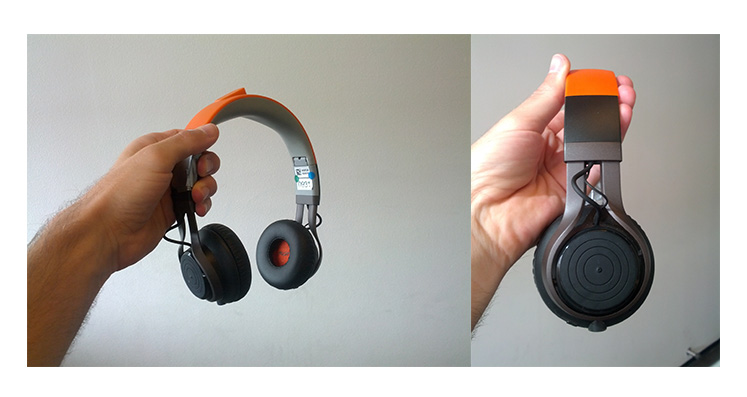
\includegraphics[width=0.9\textwidth,height=\textheight,keepaspectratio]{./Figures/headset.jpg}
		\rule{35em}{1pt}
	\caption[The Intelligent Headset]{The Intelligent Headset. A button is placed in the center of the left and right speaker (shown to the right).}
	\label{fig:headset}
\end{figure}

The headset features can be exploited through mobile applications using an included SDK targeting the iOS and Android platform (iOS SDK currently at version 1.82 and an Android SDK running verson 1.21 \footnote{Version information from 05-05-2014. Developer site: \url{https://developer.intelligentheadset.com/our-sdk/}}). The platform used in this project is Apples iOS. The main reason for using this platform is that when this project started the Intelligent Headset only provided an SDK compatible with iOS and still - though accessible for the Android platform today - the iOS SDK is running a higher version number making it more mature i.e. stable.

The SDK is implemented in the Spatial Music Menu application. The Intelligent Headset API (Application Programming Interface) provides features like reading the raw sensor data from all sensors, button events and functions for headset connectivity and 3D audio handling. An overview of the components and their communication is shown in figure \ref{fig:implementationoverview}.

\begin{figure}[t]
	\centering
		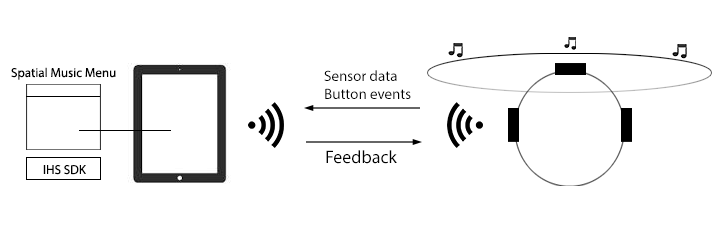
\includegraphics[width=0.9\textwidth,height=\textheight,keepaspectratio]{./Figures/implementation_overview.png}
		\rule{35em}{1pt}
	\caption[Implementation overview]{An overview of the components of the implementation and their communication}
	\label{fig:implementationoverview}
\end{figure}

\subsection{3D audio handling}
The combination of realtime sensor data and the IHS SDK functionality of setting specific audio items positions provided the required tools for implementing the audiospace. To place the audio items we used a 3D audio grid that served as a model for the audio listener and audio items, but also as a view mapping this audiospace. This 3D audio grid were defined with a virtual area size e.g. 100x100 meters.

To place audio items in a circular way we used simple geometry. We only needed the horizontal position the x and y positions of audio items were positioned by the parametric equation for a circle:

$x = cx + r * cos(a)$

$y = cy + r * sin(a)$

Where $r$ is the radius, $cx$,$cy$ the origin, and $a$ the angle from $0$ to $2\pi$ radians. Same equation were used for the audio listener position for the "carousel" zoom effect. The listeners direction were simply set by the yaw value from the gyroscope sensor data output which is the rotation value (in degrees) around the z axis. An illustration of this is showed in figure \ref{fig:circlepositions}.

\begin{figure}[t]
	\centering
		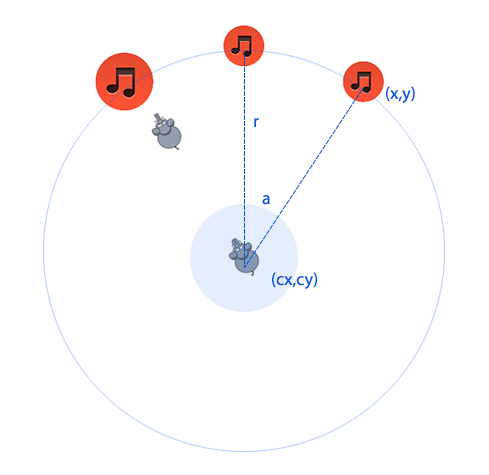
\includegraphics[width=0.6\textwidth,height=\textheight,keepaspectratio]{./Figures/circlepositions.png}
		\rule{35em}{1pt}
	\caption[Audio items positioning]{Listener and audio items positioning using circle equations.}
	\label{fig:circlepositions}
\end{figure}

\section{Music}
We used Deezer\footnote{\url{https://www.deezer.com/}} as a music provider in the implementation. Deezer is a music streaming service and provides an iOS SDK for accessing different kinds of information through their REST API e.g. track info, user playlists, albums, streaming urls, etc. This information is provided as JSON - a track item from a playlist could look like this:

\begin{lstlisting}
"tracks": {
    "data": [
      {
        "id": "1152226",
        "readable": true,
        "title": "Darkroom",
        "link": "http://www.deezer.com/track/1152226",
        "duration": "271",
        "preview": "http://cdn-preview-6.deezer.com/stream/6452dbcd46c90a70cb1147666ffd91ae-0.mp3",
        "artist": {
          "id": "1334",
          "name": "Archive",
          "link": "http://www.deezer.com/artist/1334",
          "tracklist": "https://api.deezer.com/artist/1334/top?limit=50",
          "type": "artist"
        },
        "album": {
          "id": "123427",
          "title": "Londinium",
          "cover": "https://api.deezer.com/album/123427/image",
          "tracklist": "https://api.deezer.com/album/123427/tracks",
          "type": "album"
        },
        "type": "track"
      },
\end{lstlisting}

A track represents an artist in the first level of the menu (HOME level) and by selecting a track (going up to ALBUM level) only tracks associated with the chosen tracks album id will appear. The final selection is simply the chosen album track (PLAYING TRACK level). The audio is provided by the "preview" urls which is pointing to 30 seconds preview clips. The fact that Deezer provides these preview clips of all their music was one of the main reason for using their services. This is very convinient as it is not possible to spatialise audio streams using the IHS SDK. Instead the IHS SDK is quite limited in that the only way to place sound sources in the spatial audio space is to use 16-bit wav format. Deezers preview tracks comes in MP3 format so every track needed conversion to 16-bit wav before use. 

All music information, download of preview tracks and conversion of audio was handled dynamically inside the Spatial Music Menu iOS application making it easier to add, remove and switch tracks. Basically one could add music tracks to the application by creating a Deezer playlist which is then synchronized by the iOS application. A synchronization operation is simply: 1) Getting and saving all track information from playlists including the preview tracks MP3 url; 2) download all MP3 tracks and save on device; 3) convert all tracks to 16-bit wav and save on device.


\section{Head Gestures Recognition}
To recognize head gestures we used DTW (Dynamic Time Warping) which is a well-known technique to find an optimal alignment between two time dependent sequences \cite{muller_dynamic_2007}. Due to the simple gestures (short sequences) defined in the system design we used a classic simple DTW although there exists several techniques for speeding up the algorithm \cite{muller_dynamic_2007,salvador_toward_2007,akl_accelerometer-based_2010}. 

Essentially the DTW algorithm works by compairing two sequences of length N and M. A sequence consists of observations and an observation is a set of accelerometer data from the headset. For each observation comparison a local cost is calculated and a cost matrix is created (using dynamic programming). If there exists a path (warping path) from point (1,1) to (N,M) in the cost matrix that has an overall cost that is less than a predefined cost, then there is a match. The local cost of an observation is calculated from the sum of the euclidean squared distances of each observation value. A squared euclidean distance places progressively greater weight on objects that are farther apart. The total cost is then simply the sum of all the observation distances.

A preview of such a sequence example could look like this:

\begin{lstlisting}
...
Observation: (
    "0.1245155",
    "-0.9570605",
    "0.02343822"
),
Observation: (
    "0.3266701",
    "-1.189489",
    "-0.1518601"
),
Observation: (
    "0.09228797",
    "-1.126988",
    "0.01416059"
)
...
\end{lstlisting}

The values are 3-axis accelerometer data (in order) x, y and z. An sensor observation occurs $\sim$ 30 times per second. To avoid overloading the device CPU by trying to recognise gestures for every new observation we only run the gesture recognizer for every 30 observations i.e. every second. All gesture sequences are below 100 observations so we used a window size of 100 for the testing sequence. I.e. every second the last 100 observations are tested for possible gestures.

\subsection{Training data}
Compaired with other long motion gestures e.g. running or climbing stairs, our head gestures were short events. For obtaining training data these gestures were recorded per event so a simple view containing a start/stop record button was implemented. Also to identify which class the gesture belonged to, the view had a list of labels with the specific gesture type that was to be chosen before recording the specific gesture.

The possible pause between pushing the start/stop recording button and the start or end of the actual gesture would cause some noise in the recorded data. To solve this we removed observations from the start of the recorded sequence until the difference between the start and the following observation were \textgreater 0.01. The same check was done with the end and its preceding observations. This noise cleaning was done after gestures were recorded (in memory) and the cleaned training data was saved to the device storage.


\section{iOS Application}
The Spatial Music Menu appliation were developed for an iPad Mini running iOS 7.1. As an overview and introduction of the iOS framework is out of this thesis scope - the interested reader is referred to Apples developer portal\footnote{\url{https://developer.apple.com/}} where a comprehensive documentation on the framework is available. Instead this section will focus on the application architecture, the design patterns and most the important functionality of the Spatial Music Menu.

An overview of the application architecture is shown in figure \ref{fig:apparchitecture}. The figure highlights the different relationships between application state, headset events handling, view (and audio) controller logic and persistency storage. The application aims to use iOS best practice design patterns provided by Apple\footnote{\url{https://developer.apple.com/library/ios/referencelibrary/GettingStarted/RoadMapiOS/DesignPatterns.html}} e.g. Model-View-Controller and delegation patterns.

\begin{figure}[t]
  \centering
    \includegraphics[width=\textwidth,height=\textheight,keepaspectratio]{./Figures/app-architecture.pdf}
    \rule{35em}{1pt}
  \caption[App architecture]{iOS app architecture overview}
  \label{fig:apparchitecture}
\end{figure}

\subsection{Application state management}
... Singleton approach

\subsection{Headset events handling}
...

\subsection{View controller logic}
- TODO: show screenshots of iPad 3 views

\subsection{Models and persistency storage}
...









